\chapter{Detekce jazyka}
\label{chap:detekce}

Aplikace může přijímat vstup ve~více jazycích. Jedním ze způsobů, jak uživateli zpříjemnit práci s aplikací, je použít automatický detektor jazyka. Při zadání vstupu aplikace se aplikace sama pokusí detekovat jazyk zadaného textu. Tato detekce nemusí být vždy stoprocentně správná, takže by uživatel měl mít možnost volbu jazyka manuálně změnit. Podobnou možnost nabízí uživatelům také Překladač Google\cite{googletranslate}.

Aplikace používá algoritmus založený na statistice nejčastějších N-gramů pro~daný jazyk\cite{cavnar}. Algoritmus nejprve použije velký korpus textů pro~každý detekovaný jazyk. pro~češtinu a angličtinu lze použít například korpus Wikipedie. z~tohoto korpusu získá uspořádaný seznam $K$ nejčastějších N-gramů. Při samotné detekci jazyka textu, pak samotný algoritmus získá stejný uspořádaný seznam nejčastějších N-gramů pro~vstupní text. Tento seznam pak porovnává se seznamy nejčastějších N-gramů pro~každý jazyk.

Nechť $A$ a $B$ jsou seznamy N-gramů s $K$ položkami, $A[w]$ je pořadí N-gramu $w$ v~seznamu $A$. Potom lze vzdálenost mezi seznamy $D(A,B)$ vyjádřit vztahem:

\begin{equation}
  D(A, B) = \sum_{w\,\in\,A} \begin{array}{l l} |A[w] - B[w]| & \mathrm{pokud}\ w \in B \\
  k~& \mathrm{jinak} \end{array}
\end{equation}

Na Obrázku~\ref{fig:detekce_jazyka} je ukázka porovnání dvou seznamů pomocí funkce $D(A,B)$. Trigram $na\_$ se v~seznamu B nenachází, proto dostane hodnotu $K = 4$.

Nyní pokud máme množinu $S$ všech seznamů N-gramů pro~jednotlivé jazyky a $X$ je seznam N-gramů pro~vstupní text, vrátí algoritmus jako jazyk takový jazyk, pro~který má seznam $C \in S$ minimální hodnotu $D(X, C)$.


\begin{figure}[h]
  \centering
  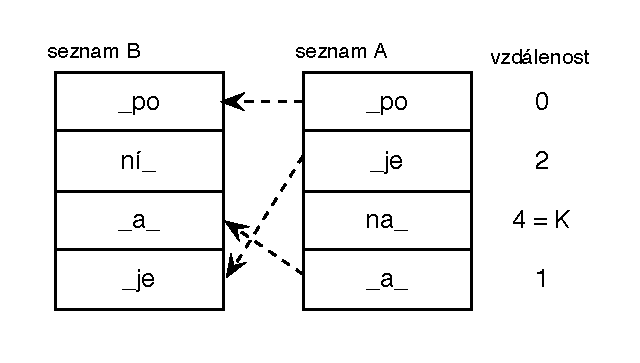
\includegraphics[width=80mm]{detekce_jazyka.eps}
  \caption{Ukázka porovnání dvou trigramových seznamů. $D(A, B) = 7$}
  \label{fig:detekce_jazyka}
\end{figure}


Naše implementace používá v~seznamech N-gramů trigramy. pro~texty delší než několik slov funguje velmi spolehlivě. pro~několikaslovné texty se může stát, že v~seznamu nejfrekventovanějších trigramů pro~vstupní text není ani jeden trigram, který by se nacházel v~seznamech pro~jednotlivé jazyky. Pak algoritmus může vrátit špatně detekovaný jazyk.

Vylepšení by jistě přineslo spolu s použitím trigramů použít i bigramy a unigramy. Také konstanta $K$ by šla zvětšit z~používané hodnoty $50$ výš. Implementace detekce jazyka ale probíhá na klientovi, takže všechna tato vylepšení algoritmu by zvýšila množství dat, která si klient musí stáhnout. Navíc uživatel má vždy možnost detekovaný jazyk manuálně změnit a typicky pracuje spíše s delšími texty. Implementace s použitím $50$ nejčastějších trigramů se tedy zdá dostačující pro~daný účel.